\chapter{METODOLOGIA}

A metodologia deste trabalho seguirá uma estrutura de etapas, indo desde o levantamento de material teórico e estudo de trabalhos relacionados até a utilização e implantação prática da aplicação apresentada. O trabalho seguirá as seguintes fases:

\section{PESQUISA BIBLIOGRÁFICA}

Será realizada uma pesquisa que visa analisar trabalhos similares realizados com robôs seguidores de linha e ROS. A pesquisa será disposta no capítulo \ref{cha:Trabalhos_relacionados}.


\section{FERRAMENTAS E MATERIAIS}

A execução e a comprovação dos resultados serão realizadas nas instalações do Laboratório de Automação, Robótica e Sistemas Inteligentes (LABIRAS), vinculado ao Instituto Federal do Piauí (IFPI), campus Teresina Central. Serão empregados recursos de eletrônica, computação e fabricação digital disponíveis no local, com destaque para a utilização do Roomba® 614 iRobot, pertencente ao laboratório.

\begin{figure}[!ht]
  \caption{\label{fig:roomba_labiras}Roomba® 614 iRobot do LABIRAS.}
  \centering
  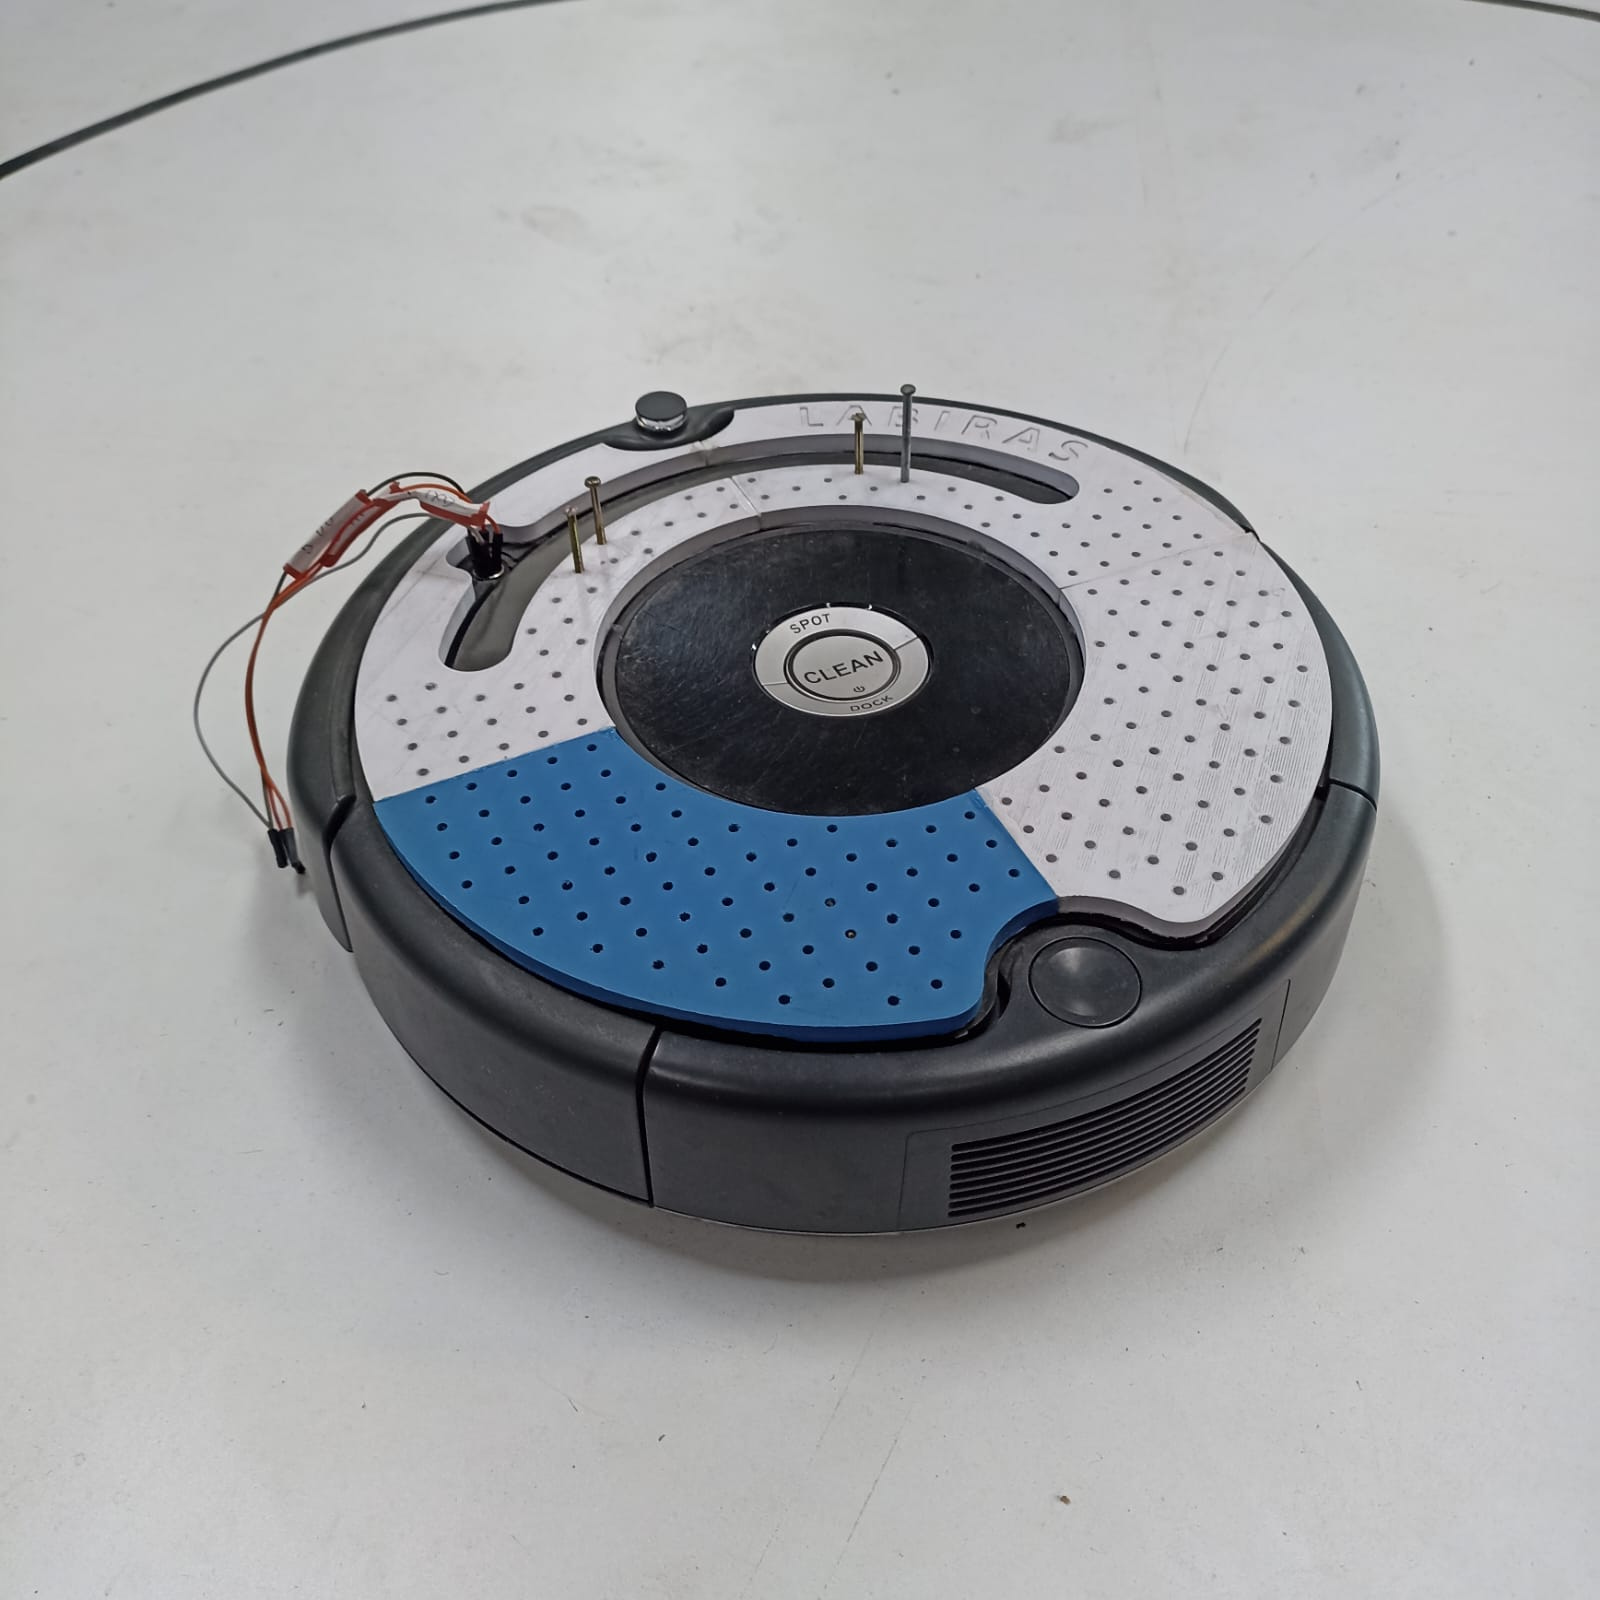
\includegraphics[scale=0.15]{figuras/roomba_labiras.jpg}
  \legend{\Fonte{Elaborado pelo autor.}}
\end{figure}

Outrossim, a proposta utilizará um módulo de 5 sensores IR BFD-1000, que consiste em um conjunto de cinco sensores infravermelhos de alta sensibilidade dispostos para a detecção precisa de linhas pretas ou brancas em superfícies, essencial para o funcionamento do robô seguidor de linha. Além disso, o módulo possui um sensor infravermelho frontal para detecção de distância e um sensor de impacto, o que amplia suas aplicações e contribui para trabalhos que envolvem navegação autônoma e evitar colisões. O BFD-1000 é compacto, de fácil aplicação, fornece sinais digitais limpos para o microcontrolador e conta com LEDs indicadores para facilitar a depuração durante o desenvolvimento. Seu uso é fundamental para garantir a precisão na leitura do trajeto, especialmente em curvas acentuadas, proporcionando maior robustez e confiabilidade ao controle do robô. Por esses motivos, este módulo é uma escolha adequada para a proposta por sua versatilidade e eficiência comprovada em robótica móvel e projetos educacionais.

\begin{figure}[!ht]
  \caption{\label{fig:modulo_ir_roomba}Módulo com 5 sensores infravermelho.}
  \centering
  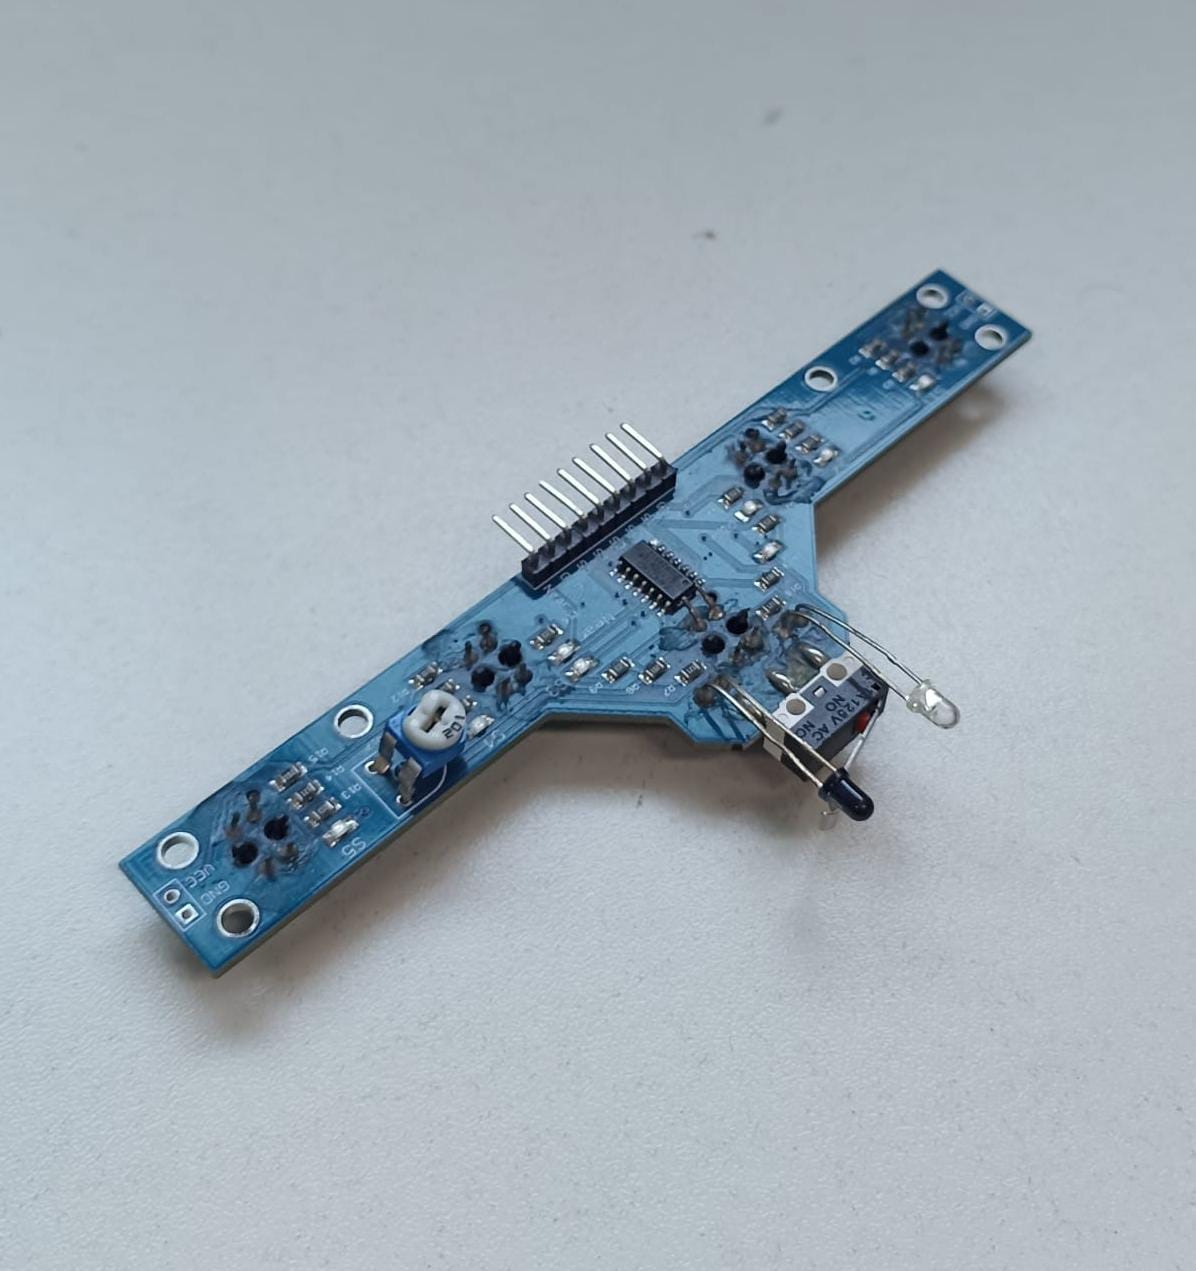
\includegraphics[scale=0.2]{figuras/sensor_IR_roomba.jpg}
  \legend{\Fonte{Elaborado pelo autor.}}
\end{figure}

% O uso do ABS permitiu a fabricação de componentes com boa rigidez estrutural e precisão dimensional, características essenciais para garantir o correto acoplamento dos motores, sensores e módulos eletrônicos da plataforma. As peças foram modeladas no software Autodesk Fusion 360, respeitando os parâmetros de montagem do sistema mecânico e dos módulos de controle. Isto posto, durante o processo de fabricação, adotaram-se parâmetros de impressão específicos para o ABS, como mesa aquecida a cerca de 110 °C e temperatura de extrusão em torno de 230 °C.

% Outrossim, o sistema de tração do projeto foi composto por quatro motores JGA25-370 com \textit{encoders} acoplados (Figura \ref{fig:motor-jga25-370}), responsáveis pelo acionamento individual de cada roda mecanum. Esses motores de corrente contínua apresentam um conjunto integrado de redutor metálico e sensor de realimentação, o que permite combinar torque elevado e controle de velocidade e posição. O \textit{encoder} de dois canais, instalado no eixo traseiro do motor, gera pulsos proporcionais à rotação do eixo, possibilitando a estimativa da velocidade angular e da distância percorrida. Além disso, o baixo consumo de corrente e a tensão nominal de operação entre 6 e 12 V tornam o modelo JGA25-370 adequado para aplicações educacionais e experimentais, proporcionando um equilíbrio entre desempenho e eficiência energética no contexto de robótica móvel.


% \begin{figure}[!ht]
%   \caption{\label{fig:motor-jga25-370}Motores JGA25-370 com \textit{encoders} acoplados.}
%   \centering
%   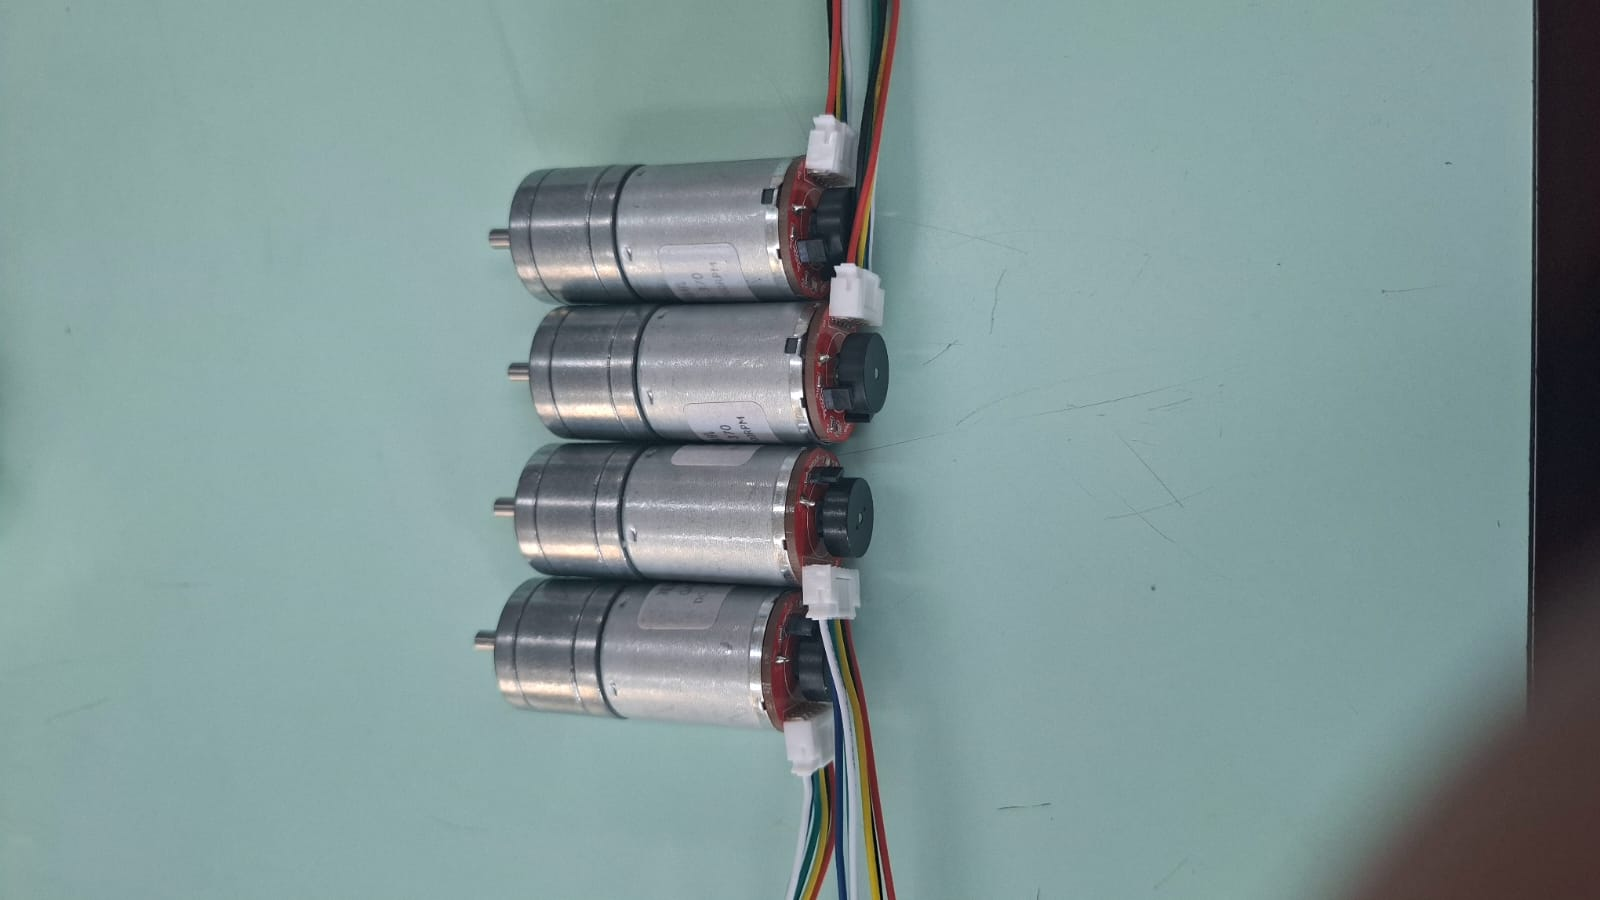
\includegraphics[scale=0.2]{figuras/motores_encoders.jpg}
%   \legend{\Fonte{Elaborado pelo autor.}}
% \end{figure}


Adicionalmente, a proposta incorpora um sistema de monitoramento e visualização topológica integrado ao ecossistema ROS 2. O objetivo desta funcionalidade é permitir que o operador acompanhe o progresso lógico do robô em tempo real, indo além da simples telemetria métrica.

Nesta abordagem, o ambiente é mapeado através de \textit{checkpoints} (pontos de controle) virtuais situados em locais estratégicos, como bifurcações e interseções da pista. Quando o sistema de percepção do robô identifica e transpõe um desses marcos, ele publica mensagens de evento informando a decisão tomada (por exemplo: "Intersecção A: Curva à Direita") e atualiza seu estado topológico. Isso permite visualizar em qual segmento específico do trajeto o veículo se encontra a cada instante, facilitando a validação do comportamento autônomo em cenários de múltipla escolha.

As plataformas robóticas móveis terrestres do LABIRAS (Figura \ref{fig:plataformas_roboticas_labiras}), baseadas no Roomba® 614, serviram como referência para a validação desta dinâmica de navegação diferencial e para a modelagem dos estados topológicos propostos.

\begin{figure}[!ht]
  \caption{\label{fig:plataformas_roboticas_labiras}Plataformas robóticas móveis terrestres do LABIRAS.}
  \centering
  \includegraphics[scale=0.15]{figuras/plataformas_roboticas_labiras.pdf}
  \legend{\Fonte{Elaborado pelo autor.}}
\end{figure}


Diante disso, o desenvolvimento do robô seguidor de linha proposto neste trabalho busca contribuir para o aprimoramento das práticas educacionais e de pesquisa no que diz respeito à utilização de robôs com essa configuração, que vem ganhando cada vez mais espaço no panorama da robótica moderna aplicada em estudos e pesquisas.



\section{SOFTWARE}

O software de controle será desenvolvido com base no ROS 2, através da linguagem de programação C++, executado no Raspberry Pi 4, como uma estação Linux. A arquitetura do sistema foi projetada para permitir a comunicação entre dois módulos distintos: o ESP32 e um Raspberry Pi 4 Model B.

O robô também será equipado com um ESP32, que será programado em C++ utilizando o Integrated Development Environment (IDE) Cursor, que possui várias extensões que auxiliam no desenvolvimento de software. Dentre essas extensões, vale ressaltar o uso da extensão PlatformIO, que auxilia o envio do algoritmos para dentro do microcontrolador, além de auxiliar no gerenciamento de bibliotecas.

Isto posto, o microcontrolador atuará como nó cliente do micro-ROS Agent, conectando-se ao servidor ROS por meio de rede Wi-Fi. Após a inicialização, o robô publica mensagens de telemetria e subscreve comandos de navegação enviados a partir de um nó de controle.

\subsection{Controle de Navegação}
O controle de navegação autônoma será executado pelo nó ROS 2 do Raspberry Pi. Este nó implementa uma malha de controle fechada baseada no algoritmo Proporcional-Integral-Derivativo (PID), responsável por corrigir a trajetória do robô em tempo real.

A lógica de funcionamento segue os seguintes passos:

\begin{enumerate}
    \item \textbf{Leitura dos Sensores:} O nó subscreverá a um tópico ROS, recebendo um vetor de dados correspondente ao estado dos 5 sensores infravermelhos do módulo BFD-1000.
    
    \item \textbf{Cálculo do Erro ($e(t)$):} Atribui-se um peso para cada sensor (ex: -2, -1, 0, 1, 2), onde 0 representa o sensor central (robô alinhado). O erro instantâneo é calculado pela média ponderada dos sensores ativos. Se o erro for negativo, o robô deve girar para a esquerda; se positivo, para a direita.
    
    \item \textbf{Algoritmo PID:} O valor de correção angular $u(t)$ é calculado pela equação discreta do PID:
    \begin{equation}
        u(t) = K_p \cdot e(t) + K_i \cdot \sum_{0}^{t} e(k) + K_d \cdot (e(t) - e(t-1))
    \end{equation}
    Onde $K_p$, $K_i$ e $K_d$ são as constantes de ganho sintonizadas experimentalmente para garantir uma resposta rápida e estável.
    
    \item \textbf{Publicação de Comando:} A saída $u(t)$ é convertida em uma mensagem do tipo \textit{geometry\_msgs/twist}. A velocidade linear ($v$) é mantida constante (ou reduzida dinamicamente em curvas acentuadas), enquanto a velocidade angular ($z$) recebe o valor de $u(t)$. Esta mensagem será publicada no tópico \textit{/piline/cmd\_vel}, instruindo os motores a realizarem a correção de trajetória necessária.
\end{enumerate}

\subsection{Monitoramento e Visualização Topológica}
Paralelamente ao PID, o sistema executará um algoritmo de detecção de padrões para identificar eventos topológicos na pista (bifurcações, cruzamentos ou marcas de fim de curso).

Ao detectar uma configuração específica de sensores (ex: todos os sensores ativos indicando um cruzamento), o robô:
\begin{enumerate}
    \item Identifica o evento como um \textit{checkpoint} lógico;
    \item Toma uma decisão de navegação, como virar à direita em uma bifurcação pré-programada;
    \item Publica um marcador visual (\textit{visualization\_msgs/Marker}) para um software como o \textit{RViz2}.
\end{enumerate}

Dessa forma, a interface gráfica exibe não apenas a posição do robô, mas desenha no mapa virtual o caminho percorrido e destaca visualmente as decisões tomadas, como setas indicando curvas ou textos informando os \textit{checkpoints} alcançados, permitindo que o operador valide a lógica de navegação em tempo real.

\section{HARDWARE}

A arquitetura eletrônica foi montada em camadas:

\begin{itemize}
	\item Camada de controle: Raspberry Pi 4 Model B, atuando como o nó de controle e processamento principal;
	\item Camada de sensoriamento: ESP32, equipado com sensores infravermelho, coletando dados dos mesmos para ajustes de direção e navegação;
	\item Camada de comunicação: módulos Wi-Fi integrados do ESP32 e do Raspberry Pi 4;
	\item Alimentação: bateria 12V.
\end{itemize}

A Figura \ref{fig:diagrama_conexoes_dispositivos} ilustra a arquitetura geral de comunicação entre os dispositivos, destacando o fluxo de dados entre a plataforma robótica (PilineBot) e a estação de visualização externa (ROS 2 Agent), eliminando a necessidade de controladores manuais dedicados.


\begin{figure}[!ht]
  \caption{\label{fig:diagrama_conexoes_dispositivos}Diagrama com a proposta de arquitetura de conexão entre os dispositivos.}
  \centering
  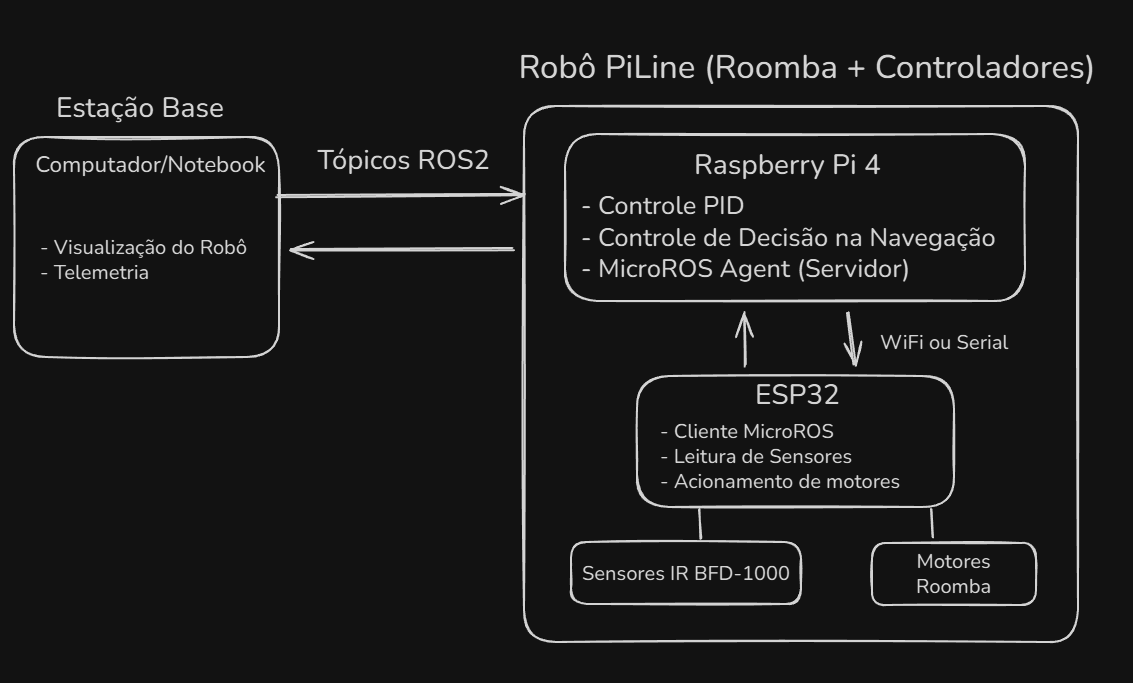
\includegraphics[scale=0.65]{figuras/proposta_conexoes_dispositivos.png}
  \legend{\Fonte{Elaborado pelo autor.}}
\end{figure}


\section{PADRONIZAÇÃO}

A padronização dos códigos e mensagens, bem como a estrutura de diretórios seguirá o modelo de packages ROS 2, conforme apresentado na Figura \ref{fig:estrutura_projeto_ros2} com base no modelo descrito pela documentação oficial ROS \cite{ros2_humble_create_package}, e os tópicos utilizam nomes normalizados (como \textit{/piline/cmd\_vel}, \textit{/piline/wheels}), de modo a facilitar a compatibilidade com outros projetos desenvolvidos no LABIRAS. Essa abordagem permite a expansão futura do sistema e integração com simuladores, como o Gazebo.


\begin{figure}[!ht]
  \caption{\label{fig:estrutura_projeto_ros2}Estrutura de projeto ROS 2.}
  \centering
  \includegraphics[scale=1]{figuras/estrutura_projeto_ros2.pdf}
  \legend{\Fonte{\citeonline{ros2_humble_create_package}.}}
\end{figure}


Para a comunicação de baixo nível dos sensores, definiu-se a estrutura de mensagem customizada, denominada aqui como \textit{wheels}, que é publicada através do tópico \textit{/piline/wheels}. Esta definição seguiu como referência o padrão das mensagens do pacote \textit{create\_msgs}, comumente utilizado em plataformas baseadas no hardware da iRobot, mas adaptada para as especificidades do robô aspirador utilizado no LABIRAS. A estrutura possui, além do cabeçalho (\textit{header}), seis campos de dados divididos simetricamente entre as rodas motrizes:

\begin{itemize}
	\item \textbf{\textit{header:}} Contém o carimbo de tempo e o quadro de referência da mensagem;
	\item \textbf{\textit{drop\_left:}} Dado booleano de segurança que indica se a roda esquerda perdeu contato com o solo (\textit{wheel drop});
	\item \textbf{\textit{encoder\_counts\_left:}} Valor acumulado da contagem do codificador incremental da roda esquerda;
	\item \textbf{\textit{velocity\_left:}} Velocidade linear instantânea da roda esquerda em mm/s;
	\item \textbf{\textit{drop\_right:}} Dado booleano de segurança que indica se a roda direita perdeu contato com o solo;
	\item \textbf{\textit{encoder\_counts\_right:}} Valor acumulado da contagem do codificador incremental da roda direita;
	\item \textbf{\textit{velocity\_right:}} Velocidade linear instantânea da roda direita em mm/s.
\end{itemize}

\section{DOCUMENTAÇÃO}

Uma documentação técnica será produzida, incluindo diagramas de blocos, fluxogramas de comunicação e instruções de compilação e operação. O objetivo é permitir que futuros pesquisadores e estudantes possam reproduzir e expandir o projeto.